\documentclass[11pt,reqno,final]{amsart}
\usepackage[font=small,margin=10pt,labelfont={bf},labelsep={space}]{caption}
\usepackage{subfig}
\usepackage{wrapfig}
\usepackage{amsmath, amssymb, epsfig}
\usepackage[scaled]{helvet} % I like Helvetica for sf
\usepackage{fourier}
\usepackage{bm}
\usepackage{color}
\usepackage{fullpage} 	% Fullpage package
%\usepackage{cite}
%\usepackage{citesort}
\newcommand{\notate}[1]{\textcolor{red}{\textbf{[#1]}}}
%\input{macros}


\newcommand{\tasos}{\text{TASOS}}
%Results
%Shortcuts
\newcommand{\hide}[1]{}
\newcommand{\R}{\mathbb{R}}
\newcommand{\E}{\mathbb{E}}
\newcommand{\N}{\mathbb{N}}
\newcommand{\Z}{\mathbb{Z}}

\newcommand{\x}{\mathbf{x}}
\newcommand{\y}{\mathbf{y}}
\newcommand{\z}{\mathbf{z}}
%\newcommand{\A}{\mathbf{A}}
\newcommand{\bi}{\mathbf{b}}
\newcommand{\ro}{\mathbf{r}}
\newcommand{\w}{\mathbf{w}}
\newcommand{\zero}{\mathbf{0}}
\newcommand{\ep}{\epsilon}
\newcommand{\de}{\delta}
\newcommand{\defby}{\overset{\mathrm{\scriptscriptstyle{def}}}{=}}
\newcommand{\bigO}{\mathrm{O}}
\DeclareMathOperator*{\argmin}{arg min}
\DeclareMathOperator*{\argmax}{arg max}
%************************************
%************************************
% The macros below are due to Tassos Zouzias
%************************************
%************************************

\newcommand{\eps}{\varepsilon}


\newcommand{\Prob}[1]{\ensuremath{\mathbb{P}\left(#1\right)}}

\newcommand{\OO}{\mathcal{O}}
\newcommand{\vol}[1]{\text{vol}(#1)}
\newcommand{\tr}{\rm{Tr}}
\newcommand{\RR}{\mathbb{R}}
\newcommand{\NN}{\mathbb{N}}
\newcommand{\reals}{\mathbb{R}}


\newcommand{\e}{\ensuremath{{\rm e}}}
\DeclareMathOperator{\EE}{\mathbb{E}}
% Variance
\newcommand{\var}[1]{\ensuremath{\mathrm{Var}(#1)}}
% Pseudo-inverse of a matrix
\newcommand{\pinv}[1]{ {#1}^\dagger}
\newcommand{\norm}[1]{\ensuremath{\left\|#1\right\|_2}}
\newcommand{\pnorm}[1]{\ensuremath{\left\|#1\right\|_p}}
\newcommand{\qnorm}[1]{\ensuremath{\left\|#1\right\|_q}}
\newcommand{\infnorm}[1]{\ensuremath{\left\|#1\right\|_\infty}}
\newcommand{\onenorm}[1]{\ensuremath{\left\|#1\right\|_1}}
\newcommand{\frobnorm}[1]{\ensuremath{\left\|#1\right\|_{\text{\rm F}}}}
% Stable rank of a matrix
\newcommand{\sr}[1]{\ensuremath{\mathrm{\textbf{\footnotesize sr}}\left(#1\right)}}
% Trace of a matrix.
\newcommand{\trace}[1]{\ensuremath{\mathrm{\textbf{tr}}\left(#1\right)}}
%\DeclareMathOperator{\trace}{trace}
% Rank of a matrix
\newcommand{\rank}[1]{\ensuremath{\mathrm{\textbf{{\footnotesize rank}}}\left(#1\right)}}
% Kernel of a matrix
%\newcommand{\ker}[1]{\ensuremath{\mathrm{\textbf{ker}}\left(#1\right)}}
% Image of a matrix
\newcommand{\im}[1]{\ensuremath{\mathrm{\textbf{Im}}\left(#1\right)}}

% Condition number of a matrix
\newcommand{\cond}[1]{\ensuremath{\mathrm{\text{cond}}\left(#1\right)}}

\newcommand{\expm}[1]{\ensuremath{\mathrm{\textbf{\footnotesize exp}}\left[#1\right]}}
\newcommand{\coshm}[1]{\ensuremath{\mathrm{\textbf{\footnotesize cosh}}\left[#1\right]}}
\newcommand{\detm}[1]{\ensuremath{\mathrm{\textbf{det}}\left(#1\right)}}
\newcommand{\sign}[1]{\ensuremath{\mathrm{\textbf{sign}}\left(#1\right)}}


% # of non-zero entries of a matrix
\newcommand{\nnz}[1]{\ensuremath{\mathrm{\textbf{\footnotesize nnz}}\left(#1\right)}}

% Diagonal Matrix
\newcommand{\diag}[1]{\ensuremath{\mathrm{\textbf{diag}}\left(#1\right)}}
% Polylog(n)
\newcommand{\polylog}[1]{\ensuremath{\mathrm{polylog}\left(#1\right)}}

\newcommand{\old}{\text{old}}
\newcommand{\new}{\text{new}}
\newcommand{\ravg}{\text{R}_{\text{avg}}}
\newcommand{\cavg}{\text{C}_{\text{avg}}}
%\newcommand{\cavg}[1]{\text{C}_{\text{avg}}(#1)}


%%% Vector and matrix operators

\newcommand{\vct}[1]{\bm{#1}}
\newcommand{\mtx}[1]{\bm{#1}}

\newcommand{\ip}[2]{\left\langle {#1},\ {#2} \right\rangle}
\newcommand{\mip}[2]{ {#1}\bullet {#2}}

\newcommand{\ignore}[1]{}

\newcommand{\Id}{\mathbf{I}}
\newcommand{\J}{\mathbf{J}}
\newcommand{\onemtx}{\bm{1}}
%\newcommand{\zeromtx}{\bm{0}}
\newcommand{\zeromtx}{\mathbf{0}}




%%%%%%%%%%%%%%%%%%%%%%%%%%%%%%%%%%%%%
\newcommand{\mat}[1]{ {\ensuremath{\mtx{#1} }}}
%%%%%%%%%%%%%%%%%%%%%%%%%%%%%%%%%%%%%

\def\gammab{{\bm{\gamma}}}
\def\kappab{{\bm{\kappa}}}
\def\sig{{\bm{\Sigma}}}
\def\sigplus{{\bm{\Sigma}^{+}}}
\def\siginv{{\bm{\Sigma}^{-1}}}
\def\bet{{\bm{\beta}}}
\def\one{{\bm{1}}}
\def\exp{\hbox{\rm exp}}
\def\col{\hbox{\rm col}}
\def\ker{\hbox{\rm ker}}
\def\ahat{{\hat\a}}
\def\p{{\mathbf p}}
\def\e{{\mathbf e}}
\def\q{{\mathbf q}}
\def\rb{{\mathbf r}}
\def\s{{\mathbf s}}
\def\u{{\mathbf u}}
\def\v{{\mathbf v}}
\def\d{{\mathbf \delta}}
\def\xhat{{\hat\x}}
\def\yhat{{\hat\y}}
\def\A{\matA}
\def\B{\matB}
\def\C{\matC}
\def\Ahat{\hat\matA}
\def\Atilde{\tilde\matA}
\def\Btilde{\tilde\matB}
\def\Stilde{\tilde\matS}
\def\Utilde{\tilde\matU}
\def\Vtilde{\tilde\matV}
\def\G{{\cl G}}
\def\hset{{\cl H}}
\def\Q{{\bm{Q}}}
\def\U{{\bm{U}}}
\def\V{{\bm{V}}}
\def\win{\hat{\w}}
\def\wopt{\w^*}
\def\matAhat{\hat\mat{A}}
\def\matA{\mat{A}}
\def\matB{\mat{B}}
\def\matC{\mat{C}}
\def\matD{\mat{D}}
\def\matE{\mat{E}}
\def\matH{\mat{H}}
\def\matI{\mat{I}}
\def\matM{\mat{M}}
\def\matP{\mat{P}}
\def\matQ{\mat{Q}}
\def\matR{\mat{R}}
\def\matL{\mat{L}}

\def\matS{\mat{S}}
\def\matT{\mat{T}}
\def\matU{\mat{U}}
\def\matV{\mat{V}}
\def\matW{\mat{W}}
\def\matX{\mat{X}}
\def\matY{\mat{Y}}
\def\matZ{\mat{Z}}
\def\matSig{\mat{\Sigma}}
\def\matOmega{\mat{\Omega}}
\def\matGam{\mat{\Gamma}}
\def\matTheta{\mat{\Theta}}
\def\w{{\mathbf{w}}}
\def\ein{{\cl E_{\text{\rm in}}}}
\def\eout{{\cl E}}
\def\scl{{\textsc{l}}}
\def\scu{{\textsc{u}}}
\def\phiu{{\overline{\phi}}}
\def\psiu{{\overline{\psi}}}
\def\phil{{\underbar{\math{\phi}}}}
\newcommand\remove[1]{}


\newcommand{\vecb}{{\vct{b} }}
\newcommand{\bc}{{\vecb_{\mathcal{R}(\matA)^\bot } }}
\newcommand{\br}{{\vecb_{\mathcal{R}(\matA) } }}

% Least squares solution of Ax = b
\def\xls{\x_{\text{\tiny LS}}}

% For rows and columns of a matrix A
\newcommand{\ar}[1]{ \matA^{(#1)}}
\newcommand{\ac}[1]{ \matA_{(#1)}}

\newcommand{\colspan}[1]{\mathcal{R}(#1)}

\usepackage{palatino}

%---------------------Listings--------------------%
\usepackage{listings}
\usepackage{color}
\definecolor{dkgreen}{rgb}{0,0.6,0}
\definecolor{gray}{rgb}{0.5,0.5,0.5}
\definecolor{mauve}{rgb}{0.58,0,0.82}
\lstset{ %
  language=Octave,                % the language of the code
  basicstyle=\footnotesize,           % the size of the fonts that are used for the code
  numbers=left,                   % where to put the line-numbers
  numberstyle=\tiny\color{gray},  % the style that is used for the line-numbers
  stepnumber=2,                   % the step between two line-numbers. If it's 1, each line
                                  % will be numbered
  numbersep=5pt,                  % how far the line-numbers are from the code
  backgroundcolor=\color{white},      % choose the background color. You must add \usepackage{color}
  showspaces=false,               % show spaces adding particular underscores
  showstringspaces=false,         % underline spaces within strings
  showtabs=false,                 % show tabs within strings adding particular underscores
  frame=single,                   % adds a frame around the code
  rulecolor=\color{black},        % if not set, the frame-color may be changed on line-breaks within not-black text (e.g. commens (green here))
  tabsize=2,                      % sets default tabsize to 2 spaces
  captionpos=b,                   % sets the caption-position to bottom
  breaklines=true,                % sets automatic line breaking
  breakatwhitespace=false,        % sets if automatic breaks should only happen at whitespace
  title=\lstname,                   % show the filename of files included with \lstinputlisting;
                                  % also try caption instead of title
  keywordstyle=\color{blue},          % keyword style
  commentstyle=\color{dkgreen},       % comment style
  stringstyle=\color{mauve},         % string literal style
  escapeinside={\%*}{*)},            % if you want to add LaTeX within your code
  morekeywords={*,...}               % if you want to add more keywords to the set
}
%-------------------------------------------------%

%%%%%%%%%%%%%%%%%%%%%%%%%%%%%%%%%%%%%%%%%%%%%%%%%%%%%%%%%%%%%%%%%%%
%%%%%%%%%%%%%%%%%%%%%%%%%%%%%%%%%%%%%%%%%%%%%%%%%%%%%%%%%%%%%%%%%%%
%%%%%%%%%%%%%%%%%%%%%%%%%%%%%%%%%%%%%%%%%%%%%%%%%%%%%%%%%%%%%%%%%%%
\usepackage{hyperref}

\usepackage[T1]{fontenc}
\usepackage[utf8]{inputenc}
\usepackage{tabularx,ragged2e,booktabs,caption}

% Place this after the backref command
\usepackage{algorithmicx}
\usepackage[ruled]{algorithm}
\usepackage{algpseudocode}

\newcommand{\floor}[1]{\lfloor #1 \rfloor}
\newtheorem{definition}{Definition}
\newtheorem{theorem}{Theorem}
\newtheorem{proposition}[theorem]{Proposition}
\newtheorem{lemma}[theorem]{Lemma}
\newtheorem{corollary}[theorem]{Corollary}
\newtheorem{question}{Question}
\newtheorem{claim}[theorem]{Claim}
\newtheorem{conjecture}[theorem]{Conjecture}
\newtheorem{observation}[theorem]{Observation}
\newtheorem{fact}[theorem]{Fact}
\newtheorem{example}{Example}
%\newtheorem{algorithm}{Algorithm}
\newtheorem{assumption}[theorem]{Assumption}
\newtheorem{remark}{Remark}
\newtheorem{problem}{Problem}

%-------------------------------------------------%


%%%%%%%%%%%%%%
% Document
%%%%%%%%%%%%%%


\title{Maximum Likelihood Estimation of Vasicek Model and \\ Calibration on Merton Jump Diffusion Using Method of Moments}
\author{Ran Zhao}
\thanks{}
\begin{document}

%%%%%%%%%%%%%%%%%%%%%%%%%%%%%%%%%%%%%%%%%%%%%%%%%%
%%%%%%%%%%%%%%%%%%%%%%%%%%%%%%%%%%%%%%%%%%%%%%%%%%
\begin{abstract}

\end{abstract}

\maketitle
%%%%%%%%%%%%%%%%%%%%%%%%%%%%%%%%%%%%%%%%%%%%%%%%%%%
%%%%%%%%%%%%%%%%%%%%%%%%%%%%%%%%%%%%%%%%%%%%%%%%%%%
%
%
%
\section{Maximum Likelihood and Vasicek Model Estimation}
\subsection{Introduction}
The Vasicek model \cite{V77} is a mathematical finance model that
describes the dynamics of interest rates. This model allows the short-term
interest rate, the spot rate, to follow a random walk, which leads
to a parabolic partial differential equation for the prices of bonds
and other interest rate derivative products. The Vasicek model referred in this paper
belongs to one factor interest rate model, where there is only one source of
randomness, the spot interest rate.

The spot rate evolution is modeled in the following stochastic differential equation:
\begin{equation} \label{vasicek_equation}
dr_t = a(b-r_t)dt + \sigma dW_t
\end{equation}
where $W_t$ is the Wiener process. $a$ can be interpreted as the speed of mean-reverting, and $b$ is the long term level of the spot rate. $\sigma$, here as
a constant, is the instantaneous volatility.

In this paper, I use the 3-month Treasury Bills rates to approximate the spot rate. The data source is Federal Reserve Bank of St. Louis website \footnote{\url{https://fred.stlouisfed.org/series/DTB3}}. Using monthly data, the 3-month Treasury Bill rates plots in the Figure~\ref{plot_rates}. From the graph, the 3-month T-bill rates display cyclical pattern, where the rate fluctuates between its long-term trend indicating by rate's moving average. However, these long term trends vary among different time period, over 1954 to 2015. Intuitively, the short term rate is tightly connected with monetary policy, and is adjusted according to the economic status. The economic cycle enhances the pattern of the short term.

\begin{figure}
  \centering
  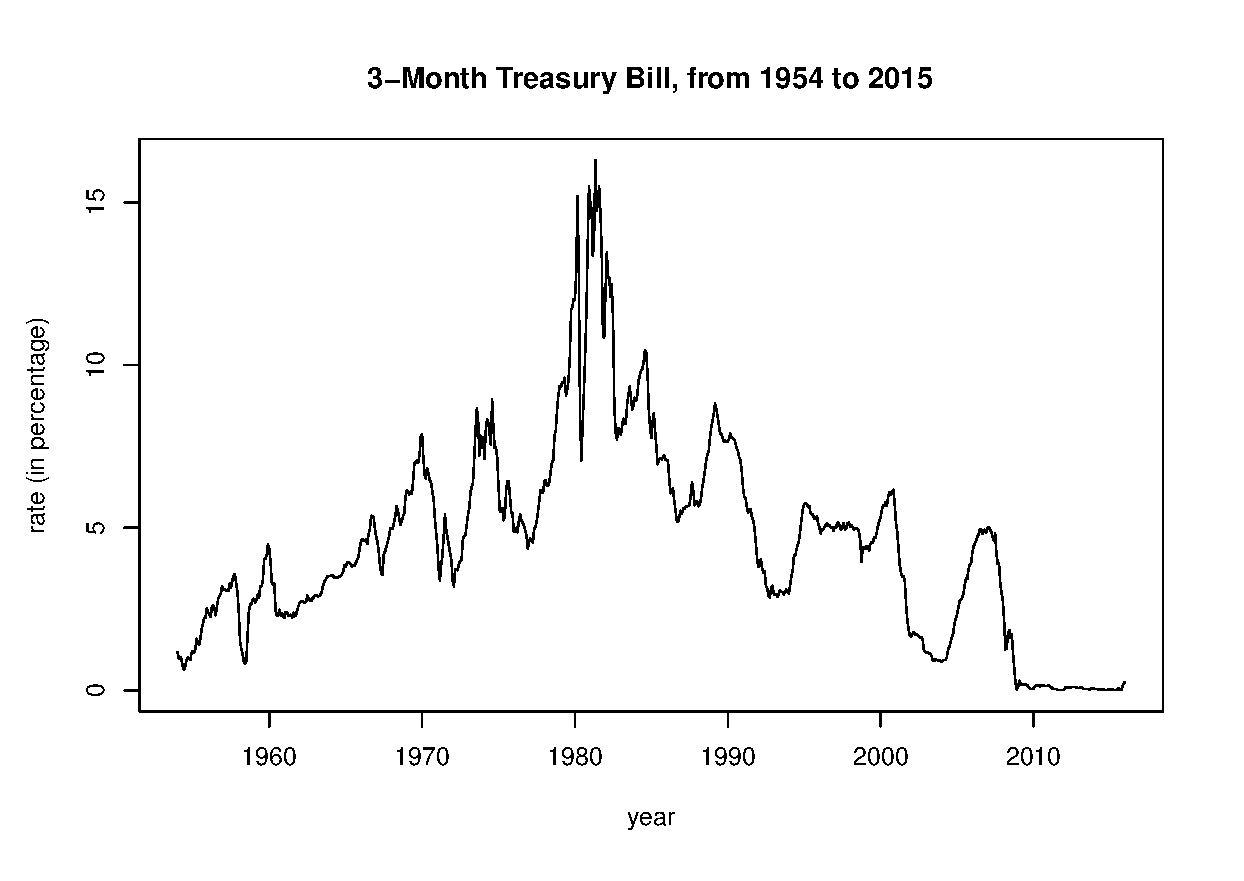
\includegraphics[scale=0.7]{plot_rates.eps}
  \caption{Monthly 3-month Treasury Bill rate at secondary market. Time period is from 1954 to 2015.}\label{plot_rates}
\end{figure}


\subsection{Discretization of Vasicek Model}
In discrete time, use $\epsilon_t$ to represent the white noise with expected value of 0 and variance of 1, evolving at time $t$. Then the discrete version of Vasicek model expresses as

\begin{eqnarray*}
\Delta r_t    &=& a(b-r_t) \Delta t + \sigma \Delta W_t \\
r_{t+1} - r_t &=& a(b - r_t) \Delta t + \sigma (W_{t+1} - W_t) \\
              &=& a(b - r_t) \Delta t + \sigma \epsilon_{t+1} \\
r_{t+1}       &=& ab\Delta t + (1 - a\Delta t) r_t + \sigma \epsilon_{t+1}
\end{eqnarray*}

Change the notation from $b$ to $\bar{X}$ to represent the mean level of rates,
from $(1-a\Delta t)$ to $\phi$ simplifying the parameter. Use $X_t$ to denote $r_t$, we yield

\begin{equation} \label{discrete_ar1}
X_{t+1} = \bar{X} (1-\phi) + \phi X_t + \sigma \epsilon_{t+1}
\end{equation}

which has the form of an AR(1) process.

\subsection{Likelihood of the AR(1) Process}
From Equation~\ref{discrete_ar1}, the conditional distribution of $X_{t+1}$ is straightforward:
\begin{equation} \label{cond_dist}
X_{t+1}|X_t \sim N(\bar{X} (1-\phi) + \phi X_t, \sigma^2)
\end{equation}
since the $\epsilon_{t+1}$ is a white noise term with mean 0 and variance 1. The information available is enough to determine $X_t$, but $\epsilon_{t+1}$ provides the source of randomness. The parameters remain to be estimated, $\mathbf{\theta}=(\bar{X},\phi, \sigma^2)'$.

The distribution of the initial value would be $X_0\sim N(\bar{X}, \frac{\sigma}{1-\phi^2})$. Hence,
\begin{eqnarray*}
f_{X_0}(x_0;\mathbf{\theta}) &=& f_{X_0}(x_0; \bar{X},\phi, \sigma^2) \\
                             &=& \frac{1}{\sqrt{2\pi}/\sqrt{\sigma^2/(1-\phi^2)}}\exp\left[ -\frac{1}{2} \frac{(x_0 - \bar{X})^2}{\sigma^2/(1-\phi^2)} \right]
\end{eqnarray*}

Next consider the conditional distribution of the second observation. According to Equation~\ref{cond_dist}, we have
$$
f_{X_1|X_0}(x_1, x_0;\mathbf{\theta}) = \frac{1}{\sqrt{2\pi\sigma^2}} \exp\left[ -\frac{1}{2} \frac{(x_1 - \bar{X} (1-\phi) - \phi x_0)^2}{\sigma^2} \right]
$$

The joint density of observations 1 and 2 is then just
$$
f_{X_2, X_1}(x_2.x_1; \mathbf{\theta}) = f_{X_1|X_0}(x_1, x_0;\mathbf{\theta}) f_{X_0}(x_0;\mathbf{\theta})
$$

In general, the value of $X_0, X_1, \ldots, X_{T-1}$ matters for $X_T$ only through the value $X_{T-1}$, and the density of observation $T$ conditional on the preceding $T-1$ observations is given by
\begin{eqnarray*}
f_{X_{T}|X_{T-1}, X_{T-2}, \ldots, X_0}(x_T|x_{T-1},\ldots, x_0;\mathbf{\theta}) &=& f_{X_{T}|X_{T-1}}(x_T|x_{T-1}; \mathbf{\theta}) \\
                             &=&  \frac{1}{\sqrt{2\pi\sigma^2}} \exp\left[ -\frac{1}{2} \frac{(x_T - \bar{X} (1-\phi) - \phi x_{T-1})^2}{\sigma^2} \right]
\end{eqnarray*}

The likelihood of the complete sample can thus be calculated as
$$
f_{X_T, X_{T-1}, \ldots, X_0}(x_T, x_{T-1}, \ldots, x_0; \mathbf{\theta}) = f_{X_0}(x_0;\theta) \cdot \prod_{t=0}^{T-1} f_{X_{t+1}|X_{t}}(x_{t+1}|x_t; \mathbf{\theta})
$$

Then the log-likelihood function (denoted by $\ell\mathbf(\theta)$) is
\begin{eqnarray*} \label{log_like_ar}
\ell(\mathbf(\theta)) &=& \log f_{X_0}(x_0;\theta) + \sum_{t=0}^{T-1} \log f_{X_{t+1}|X_{t}}(x_{t+1}|x_t; \mathbf{\theta}) \\
                      &=& -\frac{1}{2}\log 2\pi + \frac{1}{2}\log(1-\phi^2)-\frac{1}{2}\log \sigma^2 - \frac{1}{2} \frac{(1-\phi^2)(x_0-\bar{X})^2}{\sigma^2} \\
                      & & -\frac{T}{2}\log 2\pi - \frac{T}{2} \log \sigma^2 - \frac{1}{2\sigma^2} \sum_{t=0}^{T-1} [x_{t+1} - \bar{X}(1-\phi)-\phi x_t]^2 \\
                      &=& -\frac{(T+1)}{2}\log 2\pi + \frac{1}{2}\log(1-\phi^2)-\frac{(T+1)}{2}\log \sigma^2 - \frac{1}{2} \frac{(1-\phi^2)(x_0-\bar{X})^2}{\sigma^2} \\
                      & & - \frac{1}{2\sigma^2} \sum_{t=0}^{T-1} [x_{t+1} - \bar{X}(1-\phi)-\phi x_t]^2
\end{eqnarray*}

\subsection{Maximum Likelihood Estimation}
Maximum likelihood estimation (MLE) is the method of estimating model parameters given observations, by finding the parameters (here $\mathbf{\theta}$) that maximize the likelihood of the model. To optimize the likelihood function derived in Equation~\ref{log_like_ar}, use the derivative of the likelihood function with respect to the parameter set $\mathbf{\theta}$:
$$
\frac{\partial \ell\mathbf(\theta)}{\partial \mathbf{\theta}^*} = 0
$$
where again $\mathbf{\theta} = (\bar{X}, \phi, \sigma^2)'$. Here the parameter $\sigma^2$ represents the conditional variance of the short rate. The optimization requires
$$
\left\{
  \begin{array}{rcr}
    \frac{\ell\mathbf(\theta)}{\partial \bar{X}} & = & 0 \\
    \frac{\ell\mathbf(\theta)}{\partial \phi} & = & 0 \\
    \frac{\ell\mathbf(\theta)}{\partial \sigma^2} & = & 0 \\
  \end{array}
\right.
$$

Substitute the log-likelihood function in Equation~\ref{log_like_ar} into the optimization condition above yields
\begin{eqnarray*}
    \frac{\ell\mathbf(\theta)}{\partial \bar{X}} & = & -\frac{(1-\phi^2)(\bar{X}-x_0)}{2\sigma^2} + \frac{1-\phi}{\sigma^2}\sum_{t=0}^{T-1}[x_{t+1}-\bar{X}(1-\phi)-\phi x_t] = 0 \\
    \frac{\ell\mathbf(\theta)}{\partial \phi} & = & -\frac{\phi}{1-\phi^2} + \frac{\phi(x_0-\bar{X})^2}{\sigma^2} - \frac{1}{\sigma^2}\sum_{t=0}^{T-1}(\bar{X} - x_t)[x_{t+1}-\bar{X}(1-\phi)-\phi x_t] = 0 \\
    \frac{\ell\mathbf(\theta)}{\partial \sigma^2} & = & -\frac{T+1}{2\sigma^2} + \frac{(1-\phi^2)(x_0-\bar{X})^2}{2\sigma^4} + \frac{1}{2\sigma^4}\sum_{t=0}^{T-1}[x_{t+1}-\bar{X}(1-\phi)-\phi x_t]^2 = 0 \\
\end{eqnarray*}

The exact maximum likelihood estimators requires to solve the above equations. In other words, the solutions of the above equations become the exact ML estimator. However, these equations are nonlinear and difficult to solve analytically. Numerical methods and algorithms would be used in this case, and in this paper I use $\mathrm{R}$ to obtain the

\begin{table}[H]
\begin{center}
\caption{Moments comparison between theoretical and empirical ones, the model is Merton jump diffusion.}
\begin{tabular}{c|c|c|c|c|c}
  \hline \hline
	&	Full Period	&	Year 1954 to 1975	&	Year 1976 to 1981	&	Year 1982 to 2005	&	Year 2006 to 2015	\\ \hline
$\phi$	&	0.2640	&	0.3877	&	-0.8310	&	0.3341	&	-0.9664	\\
$\bar{X}$	&	0.8506	&	0.8872	&	0.7368	&	0.0443	&	0.09096	\\
$\sigma^2$	&	0.6615	&	0.2424	&	0.9135	&	0.4476	&	0.2252	\\
  \hline\hline
\end{tabular}\label{tbl::mom_comp}
\end{center}
\end{table}


\section{Merton Jump Diffusion Model Calibration}
\subsection{Introduction}
A vast of literatures have extended the Black-Scholes model~\cite{BS73} in option pricing by making more reasonable assumptions on market factors, such as the distribution of the underlying. Merton's 1976 JFE article~\cite{M76} was the first to explore jump diffusion models. The jump diffusion model is designed to address the issue of fat tails, which is observed in dynamics many asset classes. However, when the underlying can jump to any level, the market is not complete, for the reason that there are more states than assets. Merton's innovative solution lies on extra randomness due to jumps can be diversified away.

The Merton jump diffusion (MJD) model was introduced to model the asset price $S_t$, mainly the equity (stock) prices. Figure~\ref{plot_spx} plots the SPX index levels from 1954 to 2015. The data source is Bloomberg. The long term return on the equity market is tremendous. The SPX index level begins at 25 in the beginning of 1954, and reached over 1500 points around 2000 and 2006. in 2015, the SPX index level exceeds 2000 points.

\begin{figure}
  \centering
  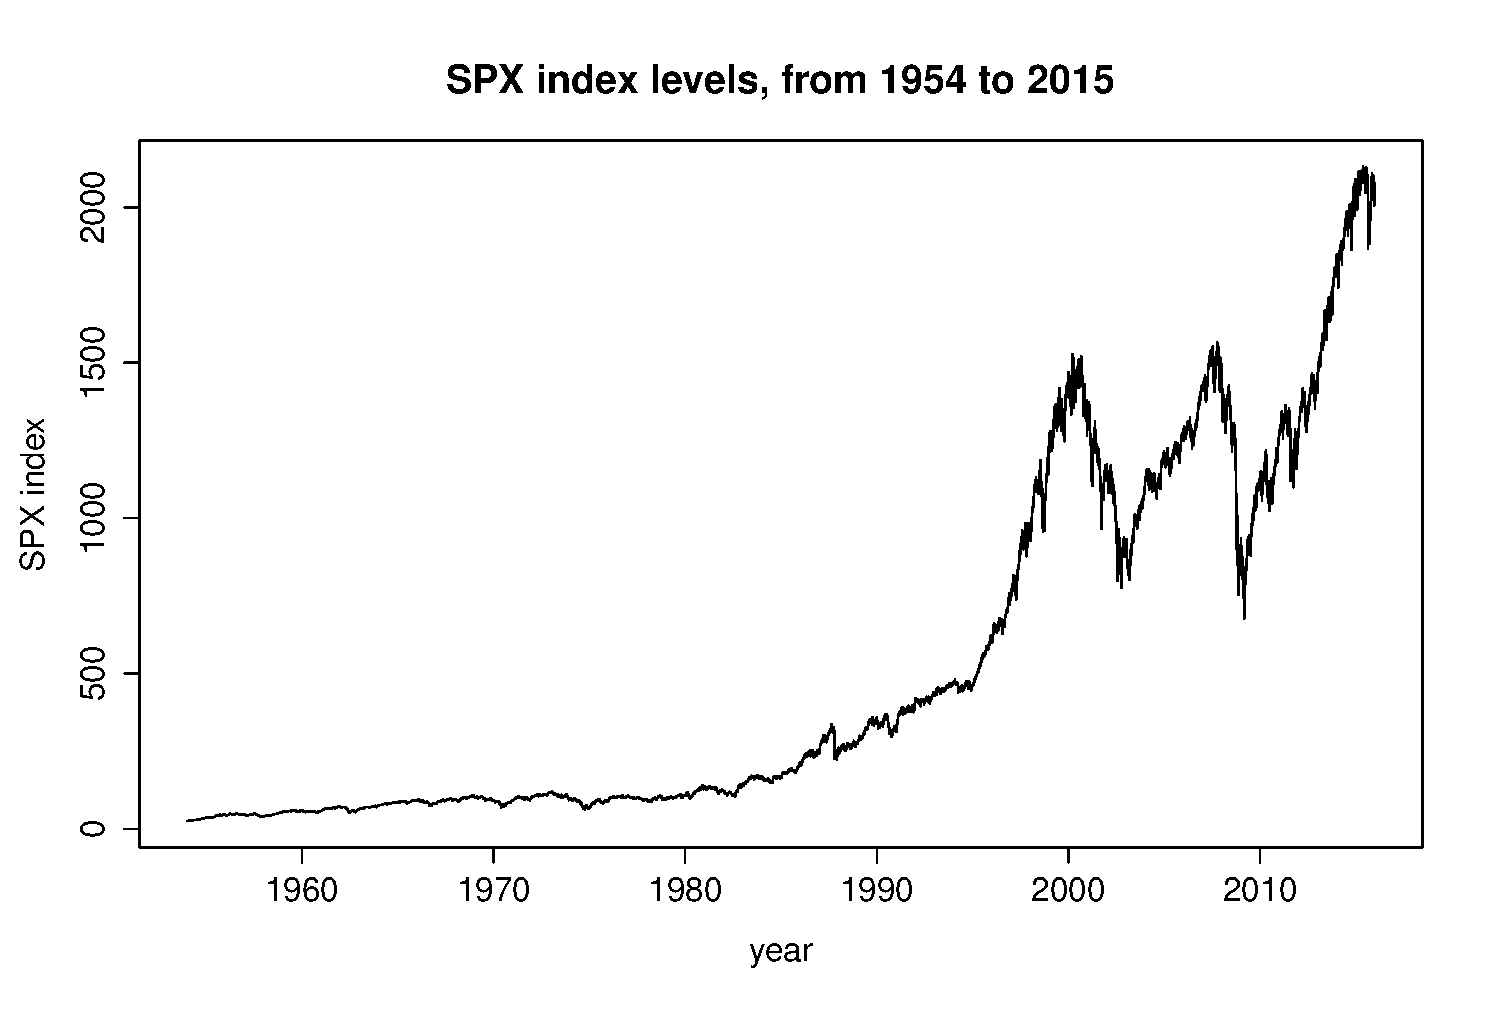
\includegraphics[scale=0.6]{plot_spx.eps}
  \caption{The SPX index levels. Time period is from 1954 to 2015.}\label{plot_spx}
\end{figure}

\subsection{Jump Diffusion Process}
Consider the dynamics of the model follows the Black-Scholes dynamics, which supposes
that the behavior of the stock price, $S_t$, is determined by the stochastic process
$$
dS_t = \mu S_t dt + \sigma S_t dW_t
$$
where $W_t$ is the Wiener process. $\mu$ and $\sigma$ are assumed to be constant and
represent the drift and diffusion, respectively.

Now consider the asset price $S_t$ with log-normal jumps $V_1, \ldots, V_j$ at random times
$\tau_1, \ldots, \tau_j$ representing the moments of jumps in a Poisson process.

The MJD model assumes the $S_t$ to follow the stochastic process:
\begin{equation} \label{jump_process}
\frac{dS_t}{S_t} = \mu dt + \sigma dW_t + d\left( \sum_{j=0}^{N_t}(V_j -1) \right)
\end{equation}

The discontinuities of the price process are described by the Poisson process $N_t$
with intensity $\lambda$ (mean arrival rate of jumps per unit time) and jump $V_j$.
And $\log V_j \sim N(\theta, \delta^2)$. The jump interprets by random variable $V$ which
transforms the price $S_t$ to $VS_t$. The difference $V-1$ is the relative price change when
a Poisson jump occurs.

Using Ito's Lemma, the strong solution of the Equation~\ref{jump_process} is
$$
S_t = S_0 \exp\left[\left( \mu - \frac{1}{2} \sigma^2 \right)t + \sigma W_t \right] \prod_{j=0}^{N_t} V_j
$$
where $S_0$ is the initial value of the stock price. Let $Y_j = \log V_j$ and rewrite
\begin{equation} \label{mjd_solution}
X_t = \log\frac{S_t}{S_0} = \left(\mu-\frac{1}{2} \sigma^2 \right)t + \sigma W_t + \sum_{j=0}^{N_t}Y_j
\end{equation}
and we assume in this paper that the processes $W_t$, $N_t$ and $Y_j$ are independent. The parameter set
of this MJD model is $\mathbf{\theta}=(\mu, \sigma^2, \theta, \delta^2, \lambda)'$.

Discretize Equation~\ref{mjd_solution} over time period $[t, t+1]$ and yield
$$
X_{t+1} = X_t + \left( \mu - \frac{1}{2}\sigma^2 \right) + \sigma \epsilon_{t+1} + \sum_{j=0}^{N_{t+1}-N_{t}}Y_j
$$
where $\epsilon_{t+1}$ is the white noise with mean 0 and variance 1.

Hence the probability density of $\Delta X_t$ can be expressed as
$$
f(x) = \sum_{n=0}^{+\infty} e^{-\lambda}\frac{\lambda^n}{n!} \frac{1}{\sqrt{2\pi(\sigma^2+n\delta^2)}} \exp\left[ -\frac{(x-\mu+\sigma^2/2 -n\theta)^2}{2(\sigma^2+n\delta^2)} \right]
$$

\subsection{Parameter Estimation with Method of Moments}
From the density function of $\Delta X_t$ (the return process), we can have
\begin{eqnarray*}
\mathbb{E}(X) &=& \sum_{n=0}^{+\infty} e^{-\lambda}\frac{\lambda^n}{n!} \int_{-\infty}^{+\infty} \frac{x}{\sqrt{2\pi(\sigma^2+n\delta^2)}} \exp\left[ -\frac{(x-\mu+\sigma^2/2 -n\theta)^2}{2(\sigma^2+n\delta^2)} \right] dx \\
\mathbb{E}[(X-\mathbb{E}(X))^k] &=& \sum_{n=0}^{+\infty} e^{-\lambda}\frac{\lambda^n}{n!} \int_{-\infty}^{+\infty} \frac{(x-\mu+\sigma^2/2 -n\theta)^k}{\sqrt{2\pi(\sigma^2+n\delta^2)}} \exp\left[ -\frac{(x-\mu+\sigma^2/2 -n\theta)^2}{2(\sigma^2+n\delta^2)} \right] dx \\
\end{eqnarray*}
for $k\geq 1$. Note that the improper integral is the central moment of order $k$ of the normal random variable with $N(\mu-(\sigma^2/2)-n\theta, \sigma^2+n\delta^2)$. Intuitively, the Poisson mixture of normals contributes to but only mean but also the variance (or volatility) term of the return process. Since the central moment with odd order becomes null for normal random variables, we use the central moments with even order to estimate the parameters. The central moments of even order is
$$
\mathbb{E}[(X-\mathbb{E}(X))^{2k}] = \frac{(2k)!}{2^k k!} \sum_{n=0}^{+\infty} e^{-\lambda}\frac{\lambda^n}{n!} (\sigma^2 + n\delta^2)^k
$$

Follow Beckers~\cite{B81} and Ball and Torous~\cite{BT85}, set $\theta$ to be 0, as to assume symmetric jumps. Using the following (lowest available) four central moments to estimate the four parameters:
\begin{eqnarray*}
\mathbb{E}(X)                       &=& \mu - \frac{\sigma^2}{2}  \\
\mathbb{E}[(X-\mathbb{E}(X))^{2}]   &=& \sigma^2 + \lambda\delta^2 \\
\mathbb{E}[(X-\mathbb{E}(X))^{4}]   &=& 3[(\sigma^2+\lambda\delta^2)^2+\lambda\delta^4] \\
\mathbb{E}[(X-\mathbb{E}(X))^{6}]   &=& 15[(\sigma^2+\lambda\delta^2)^3 + 3\lambda\delta^4(\sigma^2+\lambda\delta^2)+\lambda\delta^6] \\
\end{eqnarray*}

Then optimize the following expression to get parameter estimations:
\begin{equation} \label{opt_func}
\argmin_{\theta} g'(\theta) g(\theta)
\end{equation}
where $g(\theta)$ is the difference between theoretical moments and moments from market data. To be specific,
$$
g(\theta) = \left(
              \begin{array}{c}
                \frac{1}{N}\sum_{i=0}^N x_{i} - \mathbb{E}(X)  \\
                \frac{1}{N-1}\sum_{i=0}^N(x_{i} - \bar{X})^2 - \mathbb{E}[(X-\mathbb{E}(X))^{2}]  \\
                \frac{1}{N-1}\sum_{i=0}^N(x_{i} - \bar{X})^4 - \mathbb{E}[(X-\mathbb{E}(X))^{4}] \\
                \frac{1}{N-1}\sum_{i=0}^N(x_{i} - \bar{X})^6 - \mathbb{E}[(X-\mathbb{E}(X))^{6}] \\
              \end{array}
            \right)
$$
where $x_i$ is the $i$th observation from the market data. $N$ is the total sample size. $\bar{X}$ is the sample mean. The optimization assumes equal weights among moments.

\subsection{Calibration Results}
Optimizing (minimizing) the objective function shown in~\ref{opt_func} with help of statistical package yields the calibrated parameters as listed in Table~\ref{tbl::gmm_calibration_parameter}. The market data used for calibration contains the

\begin{table}[H]
\begin{center}
\caption{Calibrated MJD model parameters using method of moments.}
\begin{tabular}{c|c}
  \hline \hline
  % after \\: \hline or \cline{col1-col2} \cline{col3-col4} ...
  Parameters & Calibrated Value \\ \hline
  $\mu$ & 0.0004065 \\
  $\sigma^2$ & 0.0001412 \\
  $\theta$ & 0 \\
  $\delta^2$ & 0.03023 \\
  $\lambda$ & 0.001475 \\
  \hline\hline
\end{tabular}\label{tbl::gmm_calibration_parameter}
\end{center}
\end{table}

To check the goodness of fit of the MJD model calibration, we compare the empirical moments and the theoretical moments side by side in Table~\ref{tbl::mom_comp}. The first- and second- and $4^{th}$ order moments are fitted well, with relative difference less than 2\%. But $6^{th}$ order moments do not fit very well, even after adjusting the weight for $6^{th}$ order moments by the relative magnitude difference with other moments. In terms of model calibration, it seems the MJD's higher order (beyond $4^{th}$ order) moments are harder to fit. 

\begin{table}[H]
\begin{center}
\caption{Moments comparison between theoretical and empirical ones, the model is Merton jump diffusion.}
\begin{tabular}{c|c|c|c|c}
  \hline \hline 
Moments	&	Theoretical	&	Empirical	&	Diff	&	Percentage Diff	\\ \hline
1	&	3.36E-04	&	3.31E-04	&	-5.29E-06	&	-1.57\%	\\
2	&	9.66E-05	&	9.62E-05	&	-4.23E-07	&	-0.44\%	\\
4	&	2.25E-07	&	2.22E-07	&	-2.83E-09	&	-1.26\%	\\
6	&	-5.53E-08	&	5.32E-09	&	6.06E-08	&	-109.63\%	\\
  \hline\hline
\end{tabular}\label{tbl::mom_comp}
\end{center}
\end{table}


%
%
%%%%%%%%%%%%%%%%%%%%%%%%%%%%%%%%%%%%%%%%%%%%%%%%%%%
% \newpage
\bibliographystyle{plain}
\bibliography{bib}
%%%%%%%%%%%%%%%%%%%%%%%%%%%%%%%%%%%%%%%%%%%%%%%%%%%
%%%%%%%%%%%%%%%%%%%%%%%%%%%%%%%%%%%%%%%%%%%%%%%%%%%
%%%%%%%%%%%%%%%%%%%%%%%%%%%%%%%%%%%%%%%%%%%%%%%%%%%
%
%
\newpage
\section*{Appendix: Code for Vasicek model ML estimation}
%\begin{spacing}{0.9}
\lstinputlisting[language=R]{assignment1-1.R}

\newpage
\section*{Appendix: Code for Merton jump diffusion model }
\lstinputlisting[language=R]{assignment1-2.R}
%\end{spacing}

\end{document}
\endinput
